\section{Use case, resources and early-stage results}
\label{sect:motivation}

In this section, we briefly discuss a core use case for the application ApiNATOMY schematics in support of genomics and drug discovery studies. In so doing, we introduce (i) some of the key ontological and data resources required in this case, as well as (ii) early-stage results of this effort.

The domains of genomics and drug discovery are dependent on physiology knowledge, as both domains take into account the manufacture of gene products in different parts of the body and the regulated long-distance transport of molecules that interact with these products. The location of gene product manufacture (i.e. gene expression data, such as~\cite{EBI}), as well as routes associated with pharmacokinetic modeling of molecular interactors (drawn from resources such as~\cite{HMC+13}) may be usefully depicted in the form of a physiology circuitboard.

In ApiNATOMY, a physiology circuitboard schematic consists of a combination of (i) an anatomical treemap and (ii) an overlay of process graphs. In our earlier prototypes (described in~\cite{BGS12}\cite{KBK14}), templates were applied to constrain the layout of tiles in treemaps of the Foundational Model of Anatomy (FMA)~\cite{RM03} ontology, such that nesting of one tile inside another indicates that the child tile is either a part of a subclass of the parent tile. The Graphical User Interface (GUI) providing the interaction with the circuitboard allows point-and-click navigation of the treemap content. This type of interaction extends to also to involve process graphs - in this paper we report on the graphical projection of routes of (i) blood flow processes linking different regions of the human body (using data generated in~\cite{deB11}), as well as (ii) transport processes along neurons of the central nervous system (i.e. brain and spinal cord) with data obtained via the Neuroscience Information Framework~\cite{Gar+08}.

The ApiNATOMY Graphical User Interface is built from inception as a three dimensional (3D) environment. This feature facilitates interaction not only with 3D renderings of the circuit boards themselves, but also with a wide range of geometry/mesh formats for volumetric models of biological structure across scales. For instance, it is already possible to overlay Wavefront .obj data from BodyParts3D~\cite{MFT+09} as well as SWC data supported by the neuromorpho.org~\cite{Asc06} resource.

In the next sections, we discuss:
\begin{itemize}
  \item the constraining of treemap layout to generate stable anatomical treemaps,
  \item the design and overlay of routes of communication for the cardiovascular and neural systems, and
  \item the querying and 3D depiction of protein architecture schematics for the anatomical overview of gene expression data.
\end{itemize}

We arrange data in a hierarchical way starting from the large-scale views showing external and internal surfaces and organs
arranged to resemble the longitudinal section through the middle of the human body as the top-level taxonomy.
Figure~\ref{fig:application} shows the idealized radially symmetric body plan, apportioned over cylindrical regions.
This homunculus has a central longitudinal axis of rotation located in the idealized gut lumen which runs in the cephalocaudal direction.
Each of the organs in the plan is composed of multiple tissues and sub-organs, the structural information about them is obtained from the FMA ontology~\cite{RM03}. As the visualization of the full ontology may obscure the details a user is interested to see, it is essential for the visualization tool to support data filtering across multiple levels and contextual zooming into selected areas. The user should be able to create a custom view with the internal structure of the selected body parts placed in a way that simplifies the analysis of these data.

\begin{figure*}
\centering
  \subfigure[Schematic body plan]{
    \label{fig:anatomy}
    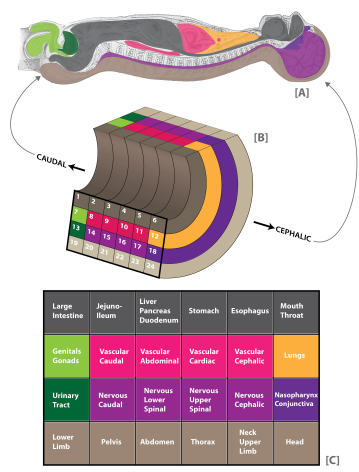
\includegraphics[width=4.3cm]{images/application.png}
  }
  \subfigure[Visualizing medical ontologies using treemaps]{
  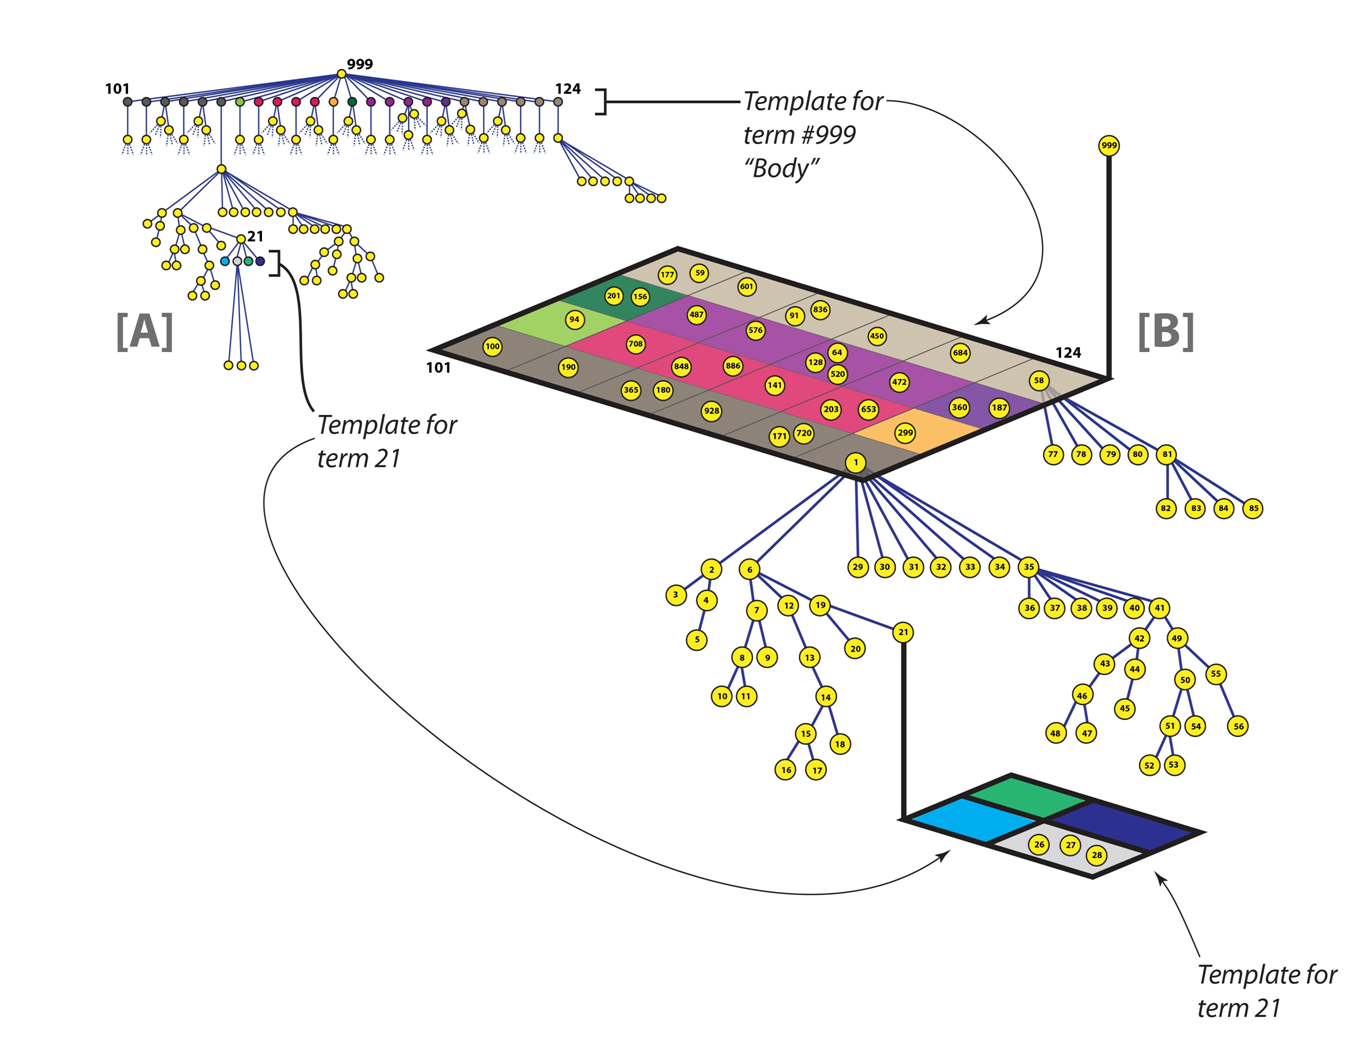
\includegraphics[width=7.3cm]{images/application1.png}
  }
  \caption{Longitudinal section through the middle of the male human body}
  \label{fig:application}
\end{figure*}

